\documentclass[11pt]{beamer}

%%%%%%%%%%%%%%%%
% Packages
%%%%%%%%%%%%%%%%
\usepackage{booktabs}
\usepackage{hyperref}		% produces hyperlinks
\usepackage{multirow}	% allows for rows that span multiple rows in tables

%%%%%%%%%%%%%%%%
% Prelims
%%%%%%%%%%%%%%%%

\usetheme[titleformat=smallcaps, progressbar=frametitle, block = fill]{metropolis}
\author{Sergio I. Garcia-Rios}
\title{Introduction to the Course}
\institute{Government 3990: Statistics in the Social Science}
\date{}



\begin{document}
\maketitle

%%%%%%%%%%%%%%%%%%%%%%%%%%%%%%%%%%%
\section{Main ideas}

%%%%%%%%%%%%%%%%%%%%%%%%%%%%%%%%%%%

\subsection{Use a sample to make inferences about the population}
\label{mi1}

%%%%%%%%%%%%%%%%%%%%%%%%%%%%%%%%%%%

\begin{frame}{1. Use a sample to make inferences about the population}
\small{
\begin{itemize}[<+->]
\item Ultimate goal: make inferences about populations
\item Caveat: populations are difficult or impossible to access
\item Solution: use a sample from that population, and use\alert{statistics} from that 
sample to make inferences about the unknown population \alert{parameters}
\item The better (more \alert{representative}) sample we have, the more reliable our 
estimates and more accurate our inferences will be
\end{itemize}

\pause


\begin{block}{Your Turn}
Suppose we want to know how many offspring female lemurs have, on average.
It's not feasible to obtain offspring data from on all female lemurs, so we use 
data from the Duke Lemur Center. We use the sample mean from these data as an 
estimate for the unknown population mean. Can you see any limitations to using data 
from the Duke Lemur Center to make inferences about all lemurs?
\end{block}
}
\end{frame}

%%%%%%%%%%%%%%%%%%%%%%%%%%%%%%%%%%%

\begin{frame}
\frametitle{Sampling is natural}

\begin{center}
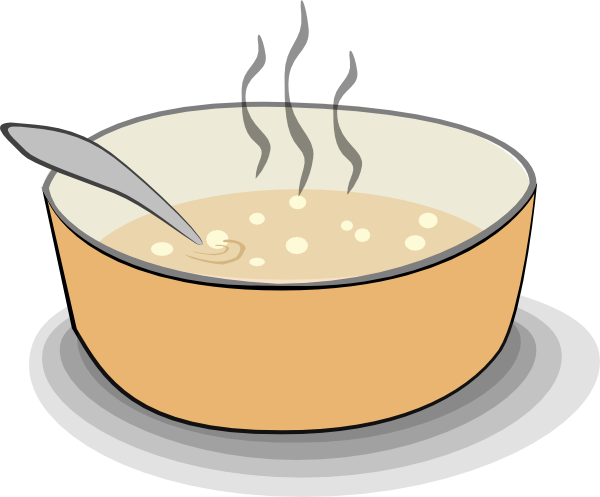
\includegraphics[width=0.3\textwidth]{figures/soup}
\end{center}

\begin{itemize}

\item When you taste a spoonful of soup and decide the spoonful you tasted isn't salty 
enough, that's \alert{exploratory analysis}

\item If you generalize and conclude that your entire soup needs salt, that's an \alert{
inference}

\item For your inference to be valid, the spoonful you tasted (the sample) needs to be 
\alert{representative} of the entire pot (the population)

\end{itemize}

\end{frame}

%%%%%%%%%%%%%%%%%%%%%%%%%%%%%%%%%%%

\subsection{Ideally use a simple random sample, stratify to control for a variable, and cluster to make sampling easier} 
\label{mi2}

%%%%%%%%%%%%%%%%%%%%%%%%%%%%%%%%%%%

%%%%%%%%%%%%%%%%%%%%%%%%%%%%%%%%%%%

\end{document}

%%%%%%%%%%%%%%%%%%%%%%%%%%%%%%%%%%%